%
% einleitung.tex -- Einleitung zum Skript ueber Differentialgleichungen
%
% (c) 2015 Prof Dr Andreas Mueller, Hochschule Rapperswil
%
\chapter*{Einleitung\label{chapter:einleitung}}
\lhead{Einleitung}
\rhead{}
Die Entdeckung der Kugelgestalt der Erde bereits im Altertum hat
klar gemacht, dass die ebene Geometrie von Euklid nur bedingt für
die Lösung von geometrischen Problemen auf der Erdoberfläche geeignet
ist.
Die Gesetze der ebenen Geometrie sind nur anwendbar, solange 
die Abmessungen des Problems klein sind im Vergleich zum Erdradius.
Sobald die Abmessungen eines geometrischen Problems vergleichbar werden
mit dem Erdradius, muss die Krümmung berücksichtigt werden.
Wir entwickeln daher in Kapitel~\ref{skript:chapter:kurven}
eine Geometrie, die auch für gekrümmte Flächen funktioniert.

Einsteins allgemeine Relativitätstheorie hat gezeigt, dass sogar das
ganze Universum als gekrümmter Raum beschrieben werden muss, um die 
Wirkung der Gravitation korrekt zu verstehen.
Doch was soll das überhaupt heissen?
Es ist ja noch einigermassen intuitiv, sich die Erdoberfläche
als gekrümmte Fläche in einem dreidimensionalen Raum vorzustellen.
Doch wo ist das Universum eingebettet?
Dies ist jedoch die falsche Frage.
Die korrekte Frage ist: wie kann man die Krümmung der Eroberfläche
nur durch Messungen innerhalb der Erdoberfläche messen?
Oder allgemeiner: wie kann man die Krümmung des Universums nur durch
Messung im Universum festzustellen.
Krümmung ist daher nicht mehr eine Eigenschaft der Einbettung eines
Raumes in einen anderen, sondern sie äussert sich als eine Abweichung
der Längenmessungen von dem, was die euklidische Geometrie verspricht.
Kapitel~\ref{skript:chapter:laengenmessung} zeigt, wie man die Längenmessung
in beliebigen Räumen mathematisieren kann.

Es zeigt sich, dass der Begriff der Krümmung auch Anwendungen ausserhalb
der Geometrie hat.
Das Fermatsche Prinzip besagt zum Beispiel, dass sich Licht immer
den kürzesten Weg sucht.
In einem inhomogenen Medium ist die Lichtgeschwindigkeit nicht
an jedem Punkt gleich, der kürzeste Weg wird daher ein Kurve sein, eine
sogenannte Geodäte.
Für einen Lichtstrahl bedeutet das, dass die Längenmessung ortsabhängig wird.
Licht sucht sich also den kürzesten Weg in einem gekrümmten Raum.
Fast alle Naturgesetze lassen sich in dieser Art als Minimalprinzip
formulieren.
Die Lösung solcher Minimalprobleme wird in
Kapitel~\ref{skript:chapter:geodaeten} dargestellt.

Eine besondere Bedeutung hat die Beschreibung des Universums als gekrümmter
Raum natürlich auch deshalb, weil diese Theorie uns ermöglicht,
die Geschichte des Universums zu rekonstruieren.
Sie hilft uns daher auch, unseren Platz im Universum besser zu
verstehen.
Dazu wird ein Modell des Universums benötigt, welches die kleinräumige
Struktur wie Galaxien und Galaxienhaufen abstrahiert und nur noch
über die grossräumige Struktur und über besonders lange Zeiträume
eine Aussage macht.
In vielen naturwissenschaftlichen Anwendungen wird ähnlich vorgegangen.
Zum Beispiel abstrahiert die Zustandsgleichung eines idealen Gases
die einzelnen Moleküle des Gases und beschreibt die Gesamtheit des
Bewegungszustands durch wenige Grössen wie Druck, Temperatur und Volumen.
Ähnlich ermöglicht Reynolds-Averaging in der Strömungsdynamik die 
komplexe Bewegung der Wirbel durch ein einfaches zusätzliches Feld und
eine leichter zu lösende gemittelte Bewegungsgleichung zu berechnen.
In den Kapiteln~\ref{skript:chapter:spezielle}
bis \ref{skript:chapter:schwarzschild} entwickeln wir zunächst die spezielle
Relativitätstheorie, verallgemeinern zur Gravitationstheorie
und studieren als Beispiel die Schwarzschild Metrik.
Die Robertson-Walker-Metrik und Kapitel~\ref{skript:chapter:kosmologie}
führt uns in Kapitel~\ref{skript:chapter:friedmann} auf die
Friedmann-Gleichungen und damit auf ein Modell für die Entwicklung des
Universums.

\begin{figure}
\centering
\includegraphics[width=\hsize]{chapters/images/20er-vorderseite.png}
%\\[10pt]
%\includegraphics[width=\hsize]{chapters/images/20er-rueckseite.png}
\caption{Vorder- und Rückseite der neuen Zwanzigernote, erschienen
im Frühjahr 2017.
Unter der Erdkugel auf der Vorderseite ist in Mikroschrift kosmologisch
interessante Information aufgedruckt, dieser Bereich ist in
Abbildung~\ref{skript:einleitung:detail} vergrössert dargestellt.
\label{skript:einleitung:noten}}
\end{figure}

\begin{figure}
\begin{center}
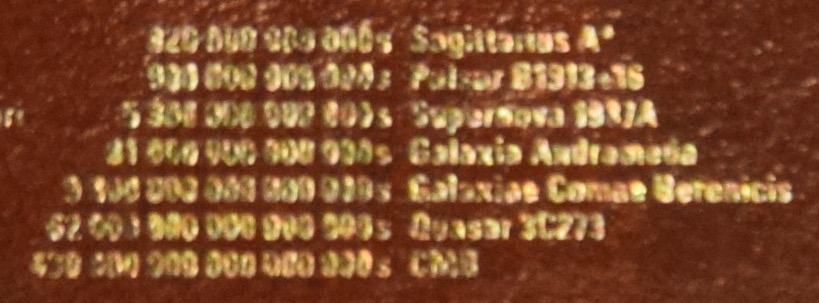
\includegraphics[width=0.7\hsize]{chapters/images/notendetail2.jpg}
\medskip

\begin{tabular}{|r|r|l|}
\hline
 Entfernung in Sekunden  &Entfernung in Jahren&Objekt                  \\
\hline
          820\,000\,000\,000&          26\,000&Sagittarius A*          \\
          980\,000\,000\,000&          31\,000&Pulsar B1913+16         \\
       5\,380\,000\,000\,000&         167\,000&Supernova 1987A         \\
      81\,000\,000\,000\,000&      2\,570\,000&Galaxia Andromeda       \\
  9\,800\,000\,000\,000\,000&    310\,000\,000&Galaxiae Comae Berenicis\\
 62\,000\,000\,000\,000\,000& 1\,960\,000\,000&Quasar 3C273            \\
430\,000\,000\,000\,000\,000&13\,600\,000\,000&CMB                     \\
\hline
\end{tabular}
\end{center}
\caption{Detail der neuen Zwanzigernote, Entfernung verschiedener
kosmologisch interessanter Objekte in Lichtsekunden und Lichtjahren.
\label{skript:einleitung:detail}}
\end{figure}

%Im zweiten Teil soll gezeigt werden, wie man durch zweckmässige
%Vernachlässigung von Details und Mittelbildung in vielen Anwendungen
%ein einfaches Modell für einen komplexen Sachverhalt bekommen kann.
%Das Modell soll dabei immer noch in der Lage sein, wesentliche
%Aspekte des ursprünglichen Problems beschreiben.
%Dieses Prinzip soll dann auf das Universum angewendet werden.
%Die Friedmann-Gleichungen erlauben uns, die Geschichte des
%Universums und sein Alter zu bestimmen.

Eine Ungewissheit bleibt aber noch, nämlich die Frage, ob das
Universum als Ganzes tatsächlich gekrümmt ist.
Die Antwort gibt es letzte mathematische Thema, nämlich die
sphärische harmonische Analyse.
Die Fouriertheorie erlaubt Funktion in einzelne Frequenzen zu
zerlegen.
Die sphärische harmonische Analyse, dargestellt in den Kapiteln
\ref{skript:chapter:multipol} und \ref{skript:chapter:kugelfunktionen}
ermöglich etwas ähnliches für Funktionen auf einer Kugel. 
Sie bestimmt die typische Grösse von Features einer solchen
Funktion, ohne dass es auf die Position derselben auf der Kugeloberfläche
ankommt.
Die Analyse des kosmischen Mikrowellenhintergrundes (cosmic microwave
background, CMB) mit der Hilfe der sphärischen harmonischen Analyse
in Kapitel~\ref{chapter:cmb} zeigt, dass das Universum im grossen
keine Krümmung hat.

Wir gelangen so zu einigen etwas überraschenden Folgerungen, die
unser Bild des Universums und seiner Geschichte in den letzten Jahren
verändert haben.
Seit Einstein war die Frage nach der grossräumigen Krümmung
und damit nach dem gesamten Energieinhalt des Universums offen.
Mittlerweile wissen wir, dass das Universum flach ist.
Das bedeutet zunächst, dass die grossräumige Geometrie doch die
einfache Geometrie ist, die wir in der Schule lernen.
Viel wichtiger ist aber, dass der Energieinhalt des Universums $0$ ist,
die Entstehung des Universums verletzt also den Energieerhaltungssatz nicht.
Universen sind gratis.

Eine weitere Folgerung ist, dass die Expansion des Universums sich
beschleunigt.
Die Galaxien, die Edwin Hubble verwendet hat, um die Expansion des
Universums zu messen, werden in einigen Milliarden Jahren so
weit entfernt sein, dass zukünftige Zivilisation nicht mehr in der
Lage sein werden, sie zu entdecken.
Die kosmische Mikrowellenstrahlung wird unmessbar schwach geworden sein.
In einer fernen Zukunft wird es also unmöglich sein, die Geschichte
des Universums zu verstehen.
Zukünftige Zivilisationen werden also die Frage nach ihrer Herkunft
prinzipiell nicht mehr beantworten können.

Während der Durchführung dieses Seminars hat die schweizerische
Nationalbank ihre neue Zwanzigernote herausgegeben, die das Thema
{\em Licht} in verschiedenen Varianten darstellt.
Zum Beispiel findet man auf der Vorderseite
(Abbildung~\ref{skript:einleitung:noten})
eine Erdkugel sowie die Sternbilder. 
Unmittelbar neben der Erdkugel sind in Mikroschrift die Entfernungen
einige kosmologisch interessanter Objekte aufgelistet
(Abbildung~\ref{skript:einleitung:detail}).
Das letzte ist der kosmische Mikrowellenhintergrund mit einer Entfernung
von gut 13.6 Milliarden Jahren.

